\LectureAnswerSection

\begin{drillsolution}{c3d1}\textbf{在已知点附近展开根式并估计余项}\par\nobreak
图\ref{c3d1q}中$h=0.01$。把$f(x)=\sqrt x$写成$x^{1/2}$，逐次应用幂函数求导法则：
\begin{align*}
f'(x)&=\frac12x^{-1/2}=\frac1{2\sqrt x},\\
f''(x)&=\frac12\left(-\frac12\right)x^{-3/2}
=-\frac1{4x^{3/2}},\\
f'''(x)&=-\frac14\left(-\frac32\right)x^{-5/2}
=\frac3{8x^{5/2}}.
\end{align*}
在四处代入得到 $f(4)=2$、$f'(4)=1/4$、$f''(4)=-1/32$，所以二阶展开为
\[
 \sqrt{4+h}=2+\frac h4-\frac{h^2}{64}+R_2,
\]
代入$h=0.01$，依次计算$h/4=0.0025$、$h^2/64=0.0000015625$，得到$\sqrt{4.01}\simeq2.0024984375$。前面已求得$f'''(x)=3/(8x^{5/2})$；它在正半轴随$x$增加而减小，所以在$[4,4.01]$上的最大值为$f'''(4)=3/(8\cdot32)=3/256$。按拉格朗日余项，
$|R_2|\le(3/256)h^3/3!=h^3/512=1.953125\times10^{-9}$。
\fig{c3d1s}{放大余项与其严格上界之比，整个区间都在一以下}{\begin{tikzpicture}
\draw[axis](0,0)--(4.8,0)node[right]{$h$};\draw[axis](0,0)--(0,2.6)node[above]{$R_2/(h^3/512)$};\fill[blue!7](0,0)rectangle(4,2);\draw[red,dashed](0,2)--(4.2,2)node[right]{上界 $1$};\draw[world]plot coordinates{(0.00000,2.0000000) (0.05000,1.9804692) (0.10000,1.9609392) (0.15000,1.9414101) (0.20000,1.9218818) (0.25000,1.9023544) (0.30000,1.8828279) (0.35000,1.8633022) (0.40000,1.8437773) (0.45000,1.8242533) (0.50000,1.8047302) (0.55000,1.7852079) (0.60000,1.7656865) (0.65000,1.7461659) (0.70000,1.7266462) (0.75000,1.7071273) (0.80000,1.6876093) (0.85000,1.6680922) (0.90000,1.6485759) (0.95000,1.6290604) (1.00000,1.6095458) (1.05000,1.5900321) (1.10000,1.5705192) (1.15000,1.5510071) (1.20000,1.5314960) (1.25000,1.5119856) (1.30000,1.4924761) (1.35000,1.4729675) (1.40000,1.4534597) (1.45000,1.4339528) (1.50000,1.4144468) (1.55000,1.3949415) (1.60000,1.3754372) (1.65000,1.3559337) (1.70000,1.3364310) (1.75000,1.3169292) (1.80000,1.2974282) (1.85000,1.2779281) (1.90000,1.2584289) (1.95000,1.2389305) (2.00000,1.2194330) (2.05000,1.1999363) (2.10000,1.1804404) (2.15000,1.1609454) (2.20000,1.1414513) (2.25000,1.1219580) (2.30000,1.1024656) (2.35000,1.0829740) (2.40000,1.0634833) (2.45000,1.0439934) (2.50000,1.0245044) (2.55000,1.0050162) (2.60000,0.9855289) (2.65000,0.9660424) (2.70000,0.9465568) (2.75000,0.9270720) (2.80000,0.9075881) (2.85000,0.8881050) (2.90000,0.8686228) (2.95000,0.8491414) (3.00000,0.8296609) (3.05000,0.8101813) (3.10000,0.7907025) (3.15000,0.7712245) (3.20000,0.7517474) (3.25000,0.7322711) (3.30000,0.7127957) (3.35000,0.6933212) (3.40000,0.6738474) (3.45000,0.6543746) (3.50000,0.6349026) (3.55000,0.6154314) (3.60000,0.5959611) (3.65000,0.5764917) (3.70000,0.5570230) (3.75000,0.5375553) (3.80000,0.5180884) (3.85000,0.4986223) (3.90000,0.4791571) (3.95000,0.4596928) (4.00000,0.4402293)};
\node[left]at(0,0){$.998$};\node[left]at(0,1){$.999$};\node[left]at(0,2){$1.000$};\node[below]at(0,0){$0$};\node[below]at(4,0){$.01$};\node at(2,-.8){纵轴只显示 $[.998,1]$，$h=0$ 取极限};
\end{tikzpicture}}



\par\medskip\Needspace{4\baselineskip}\noindent\textbf{以严格余项界确定小角允许范围}\par\nobreak
图 \ref{c3d1s}放大显示余项与上界的比值：它为正且小于 $1$，所以实际值在二阶近似上方，但增量不超过 $h^3/512$。这个界来自三阶导数，不能用保留的小数位数替代。对正弦在零点保留到二阶，常数、二次项均为零，三阶导数为 $-\cos\theta$、绝对值不超过一，因此余项界为 $|\sin\theta-\theta|\le|\theta|^3/3!$。再除以 $|\theta|>0$，得到
$|\sin\theta-\theta|/|\theta|\le\theta^2/6\le1/600$；零点以极限补充为零。这里误差的比较基准是 $\theta$，不是 $\sin\theta$。
\end{drillsolution}
\begin{drillsolution}{c3d2}\textbf{沿内法线把圆轨道曲率代入折射率梯度}\par\nobreak
令 $\delta=n(r_0)-1>0$。先对题给指数逐层求导：$n'(r)=\delta\e^{-(r-r_0)/b}\,[-1/b]$。在图\ref{c3d2q}的地表位置代入 $r=r_0$，得到 $n(r_0)=1+\delta$、$n'(r_0)=-\delta/b$；光线向折射率较大的内层弯曲。半径 $r_0$的圆形光路要求内法线曲率为 $1/r_0$，代入题给曲率关系，
\[\frac1{r_0}=-\frac{n'(r_0)}{n(r_0)}
 =\frac{\delta}{b(1+\delta)}.\]
\fig{c3d2s}{局部切向传播时的内法线曲率}{\begin{tikzpicture}
\draw[world](0,0)arc(0:70:1.7);\coordinate(P)at(0,0);\draw[ray,blue](P)--(0,1.3)node[above]{切向};
\draw[force,red](P)--(-1,0)node[left]{内法线};\node[below right]at(P){$P$};
\end{tikzpicture}}



\par\medskip\Needspace{4\baselineskip}\noindent\textbf{解出折射率增量并换算密度}\par\nobreak
图\ref{c3d2s}标明内法线方向，所以曲率取正。将等式两边乘正数 $br_0(1+\delta)$，再移项：
\[b(1+\delta)=r_0\delta,\qquad
b=(r_0-b)\delta,\qquad
\delta=\frac b{r_0-b}.\]
$n-1$与密度成正比，比较的应是折射率增量，而非两个接近一的折射率本身。先把 $r_0=6400\,\mathrm{km}$换成 $6.4\times10^6\,\mathrm m$，再与实际增量0.0003相比，得到
\[\frac{\rho_{\rm req}}{\rho_{\rm act}}
 =\frac{\delta}{0.0003}
 =\frac{8772}{(6400000-8772)\,0.0003}
 \simeq\boxed{4.575}.\]
若在曲率式中预先将 $1+\delta$近似为一，会得到约4.57；完整表达式则明确保留了这一步近似的位置。


\par\medskip\Needspace{4\baselineskip}\noindent\textbf{用任意径向扰动独立核验光路条件}\par\nobreak
还可用光程驻值独立核验圆形光路的条件，其作用是解释曲率条件的来由。取极角 $\phi$为参数，将邻近路径写成 $r(\phi)=r_0+\epsilon\eta(\phi)$，其中 $\eta$为光滑的周期函数。路径微元为
\[\dd s=\sqrt{r^2+(\dd r/\dd\phi)^2}\dd\phi
 =[r_0+\epsilon\eta(\phi)]\dd\phi+O(\epsilon^2).\]
导数平方只贡献二阶小量；折射率的一阶展开为
\[n(r)=n(r_0)+\epsilon n'(r_0)\eta(\phi)+O(\epsilon^2).\]
两式相乘，沿一周积分，得到光程的一阶变化
\[\delta\mathcal L=\epsilon\int_0^{2\pi}
 [n(r_0)+r_0n'(r_0)]\eta(\phi)\dd\phi.\]
\fig{c3d2variation}{路径略向外移时，长度增加而折射率减小}{\begin{tikzpicture}
\draw[blue,world](0,0)circle(1.5);\draw[red,dashed](0,0)circle(1.9);
\draw[guide](0,0)--(35:1.9);\draw[dim](35:1.5)--(35:1.9)node[right]{$\epsilon\eta$};
\node at(0,-2.4){蓝：$r_0$\quad 红：邻近路径};
\node[below left]at(0,0){$O$};
\end{tikzpicture}}
图\ref{c3d2variation}中路径向外移动时，几何长度增加、折射率减小。

要使任意小扰动下的一阶变化为零，二者须满足 $n(r_0)+r_0n'(r_0)=0$，即 $-n'(r_0)/n(r_0)=1/r_0$，与前面使用的曲率条件相同。两种方法由此共同核验了圆形光路的条件和弯曲方向；候选光路的扰动稳定性还需进一步检查二阶变化。
\end{drillsolution}
\begin{drillsolution}{c3d3}\textbf{列出驻点、端点并逐一比较函数值}\par\nobreak
图\ref{c3d3q}给出的 $f(x)=x^3-3x$在闭区间 $[-2,3]$连续，故全局最值一定存在。先求导并解出内部驻点：
\[f'(x)=3x^2-3=3(x-1)(x+1)=0,
\qquad x=-1,1.\]


\par\medskip\Needspace{4\baselineskip}\noindent\textbf{按单调区间收集全部候选点并比较}\par\nobreak
导数在 $[-2,-1]$为正，在 $[-1,1]$为负，在 $[1,3]$为正；这三个单调区间覆盖题设区间，所以只需比较它们的边界 $-2,-1,1,3$。逐项代入原函数，
\[f(-2)=-8+6=-2,\quad f(-1)=-1+3=2,\]
\[f(1)=1-3=-2,\qquad f(3)=27-9=18.\]
\fig{c3d3s}{端点与驻点都要比较，局部极大不保证全局最大}{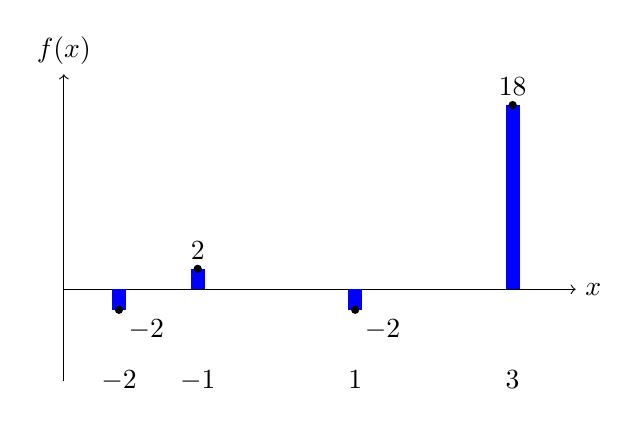
\begin{tikzpicture}[x=1cm,y=.13cm]
\draw[->](-2.7,0)--(3.8,0)node[right]{$x$};\draw[->](-2.7,-9)--(-2.7,21)node[above]{$f(x)$};
\foreach \x/\y in {-2/-2,-1/2,1/-2,3/18}{\draw[blue,line width=5pt](\x,0)--(\x,\y);\fill(\x,\y)circle(1.5pt);\node[below]at(\x,-7){$\x$};}
\node[below right]at(-2,-2){$-2$};\node[below right]at(1,-2){$-2$};\node[above]at(-1,2){$2$};\node[above]at(3,18){$18$};
\end{tikzpicture}}
由图\ref{c3d3s}的四个候选值，最大值为 $18$，在 $x=3$取得；最小值为 $-2$，在 $x=-2,1$两处取得。内部驻点 $x=-1$虽由增转减，是局部极大点，其函数值2却小于右端点的18。端点无需满足 $f'=0$，因此只列驻点不能完成闭区间最值问题。
\end{drillsolution}
\begin{drillsolution}{c3d4}\textbf{利用轴端点的正交关系求曲率}\par\nobreak
先在图\ref{c3d4q}的固定直角坐标中求一般时刻的分量。$A,B,\omega$保持不变，每次时间求导都带上内层导数$\dd(\omega t)/\dd t=\omega$：
\begin{align*}
v_x&=A[-\sin(\omega t)]\omega=-A\omega\sin\omega t,\\
v_y&=B\cos(\omega t)\omega=B\omega\cos\omega t,\\
a_x&=-A\omega\cos(\omega t)\omega=-A\omega^2\cos\omega t,\\
a_y&=B\omega[-\sin(\omega t)]\omega=-B\omega^2\sin\omega t.
\end{align*}
现在代入$t=0$，有$\bm v=(0,B\omega)$、$v=B\omega$，$\bm a=(-A\omega^2,0)$、$|\bm a|=A\omega^2$。两矢量垂直，加速度全为法向，因此
\[
\rho=\frac{v^2}{|\bm a|}
=\frac{B^2\omega^2}{A\omega^2}=\frac{B^2}{A}.
\]
\fig{c3d4s}{轴端点可以直接用全部加速度求曲率}{\begin{tikzpicture}[scale=.85]
\fill(0,0)circle(2pt)node[below right]{$P(A,0)$};\draw[force,blue](0,0)--(0,1.5)node[above]{$B\omega$};\draw[force,red](0,0)--(-1.7,0)node[left]{$A\omega^2$};
\end{tikzpicture}}



\par\medskip\Needspace{4\baselineskip}\noindent\textbf{在一般位置分离切向与法向加速度}\par\nobreak
图\ref{c3d4s}的垂直关系只在该类特殊位置成立。对一般位置，使用上面逐分量求得的速度和加速度计算点积。
点积为
$\bm v\cdot\bm a=\omega^3(A^2-B^2)\sin\omega t\cos\omega t$，
速率为$\omega\sqrt{A^2\sin^2\omega t+B^2\cos^2\omega t}$。由于$v^2=\bm v\cdot\bm v$，两边对时间求导得到$2v\dot v=2\bm v\cdot\bm a$。在本题$v>0$，因此切向加速度$a_\tau=\dot v=(\bm v\cdot\bm a)/v$，即
\[
 a_\tau=\frac{\bm v\cdot\bm a}{v}
 =\frac{\omega^2(A^2-B^2)\sin\omega t\cos\omega t}
 {\sqrt{A^2\sin^2\omega t+B^2\cos^2\omega t}}.
\]
在 $\omega t=\pi/4$ 时，分子中的 $\sin\omega t\cos\omega t=1/2$，分母根式为 $\sqrt{(A^2+B^2)/2}$，化简后为
$\omega^2(A^2-B^2)/\sqrt{2(A^2+B^2)}>0$。
所以恒定参数角速度下，椭圆上的速率正在增加；只有 $A=B$ 的圆才处处无切向加速度。

% thirty-c3-ellipsecomponents

\par\medskip\Needspace{4\baselineskip}\noindent\textbf{由速度与加速度的叉积求法向分量}\par\nobreak
为补全一般位置的分解，令 $\phi=\omega t$、
$D=A^2\sin^2\phi+B^2\cos^2\phi$。平面运动的叉积仅有垂直纸面的分量，逐项计算为
\begin{align*}
(\bm v\times\bm a)_z
 &=(-A\omega\sin\phi)(-B\omega^2\sin\phi)
 -(B\omega\cos\phi)(-A\omega^2\cos\phi)\\
 &=AB\omega^3(\sin^2\phi+\cos^2\phi)=AB\omega^3.
\end{align*}
因切向部分与 $\bm v$平行，只有法向部分进入叉积。由 $|\bm v\times\bm a|=v a_n$，可得
\[a_n=\frac{AB\omega^2}{\sqrt D},\qquad
\rho=\frac{v^2}{a_n}=\frac{D^{3/2}}{AB}.\]
\fig{c3d4components}{一般位置先分解加速度，再用法向分量求曲率}{\begin{tikzpicture}
\coordinate(P)at(0,0);\coordinate(T)at(-.842,.459);
\coordinate(N)at(-.714,-1.308);\coordinate(A)at(-1.556,-.849);
\draw[guide](T)--(A)--(N);
\draw[flow,blue](P)--(T)node[above left]{$a_\tau\bm e_\tau$};
\draw[flow,red](P)--(N)node[below]{$a_n\bm e_n$};
\draw[flow](P)--(A)node[left]{$\bm a$};
\fill(P)circle(1.4pt)node[right]{$P$};
\end{tikzpicture}}
图\ref{c3d4components}的两分量相互垂直；总加速度的大小应满足
$|\bm a|^2=a_\tau^2+a_n^2$。在 $\phi=\pi/4$处，
\[a_n=\frac{\sqrt2AB\omega^2}{\sqrt{A^2+B^2}},\qquad
a_\tau=\frac{(A^2-B^2)\omega^2}{\sqrt{2(A^2+B^2)}}.\]
两式平方相加，分子为
$4A^2B^2+(A^2-B^2)^2=(A^2+B^2)^2$，所以总量为
$\omega^4(A^2+B^2)/2$，与直接求 $a_x^2+a_y^2$相同。只有先确认 $a_\tau=0$，才能用总加速度代替法向加速度；轴端点的简便算法不应直接套到整条椭圆上。
\end{drillsolution}
